
%(BEGIN_QUESTION)
% Copyright 2011, Tony R. Kuphaldt, released under the Creative Commons Attribution License (v 1.0)
% This means you may do almost anything with this work of mine, so long as you give me proper credit

Sketch the shape and size of the first Fresnel zone ($n=1$) between these two antennas, using the grid as a guide.  Assume a signal frequency of 50 MHz, and each grid square representing 5 meters of distance.  Your sketch needs to be accurate to within $\pm$ 1/2 square ($\pm$ 2.5 meters) of the true Fresnel zone envelope at all points:

$$\includegraphics[width=15.5cm]{i03614x01.eps}$$

Also, calculate this Fresnel zone's maximum radius.

\vskip 10pt

$r_{max}$ = \underbar{\hskip 50pt} m

\underbar{file i03614}
%(END_QUESTION)





%(BEGIN_ANSWER)

Half-credit for reasonably accurate sketch (within 1/2 square of answer at all points), and half credit for correct maximum radius answer.

$$\includegraphics[width=15.5cm]{i03614x02.eps}$$

$r$ = 5.337 m at $d_1$ = 5 m \hskip 30pt $r$ = 7.346 m at $d_1$ = 10 m

\vskip 10pt

$r_{max}$ = \underbar{\bf 12.243} m

%(END_ANSWER)





%(BEGIN_NOTES)

{\bf This question is intended for exams only and not worksheets!}

%(END_NOTES)


